\documentclass[11pt]{article}
\usepackage[utf8]{inputenc}
\usepackage[T1]{fontenc}
\usepackage[english]{babel}
\usepackage{amsmath,amssymb}
\usepackage{booktabs}
\usepackage{geometry}
\geometry{margin=2.5cm}
\usepackage{hyperref}
\usepackage{pgfplots}
\pgfplotsset{compat=1.17}

\title{Memory versus generalization at micro scale:\\ does dialectical decomposition of a vault help a micro-model?\\ \large (an honest negative result)}
\author{Arkadiusz Słota \\ \textbf{Slayer} collective \\ \texttt{github.com/slayerlabs/micro-models}}
\date{June 2026}

\begin{document}
\maketitle

\begin{abstract}
On the author's Obsidian knowledge base (813 dialectical notes, $\sim$3 MB, Polish) we test two things: whether a
micro-GPT trained \emph{from scratch} \textbf{generalizes} beyond an $n$-gram, and whether a \textbf{deterministic
dialectical decomposition} (the AST-T2 schema: Thesis/Gist $\cdot$ Argumentation $\cdot$ Assumptions $\cdot$
Synthesis $\cdot$ Links) builds better representations than raw text. On a \emph{shared} raw held-out set (82
notes) we measure bits/char: \textbf{$n$-gram $2.05$ $<$ GPT-raw $2.11$ $<$ GPT-decomp $2.15$} (8000 steps, near
convergence). Both falsifiable gates come out \textbf{negative but robust}: the $n$-gram \emph{beats} the
transformer (memory $\geq$ generalization at this scale), and decomposition does \emph{not} help (a stable
$\sim$0.035 bits/char penalty from off-distribution evaluation). After more training (3000$\to$8000 steps) the gap
to the $n$-gram narrowed $0.45\!\to\!0.10$ --- the 3000-step result was an \textbf{undertraining artifact} that we
control for. We explain this with information theory (under-data'd, low-entropy repetitive corpus) and the
memory/generalization trade-off; the mechanism (attention, gradient descent) works fine --- the model learns
$55\times$ over random. We argue the principled redirection is \textbf{non-parametric memory} (kNN-LM) and adapting
pretrained models, not training a micro-model from scratch. This is also a \emph{second} data point confirming the
strength of $n$-grams on repetitive corpora.
\end{abstract}

\section{Introduction}
We care about \emph{micro-models} --- networks small enough to understand end to end and train in minutes --- and a
practical question: can a structured knowledge base (an Obsidian vault written dialectically: Goal $\to$ Thesis
$\leftrightarrow$ Antithesis $\to$ Synthesis) be \emph{turned into a model} that carries that knowledge? Retrieval
over notes (RAG, including link-graph-aware GraphRAG \cite{graphrag}) is by now solved and commoditized; less
explored is the other end: whether a \emph{generative} model trained \emph{from scratch} on such a base learns
anything beyond memory, and whether the authored dialectical structure is a useful training signal. Next-token
prediction is the shared objective from $n$-grams to transformers \cite{nplm,vaswani}; we work at its smallest
practical end and --- following the Slayer collective's principles (hard measurement, explicit cost, no
benchmaxxing) --- we report a negative result.

\paragraph{Contributions.} (1) A deterministic vault decomposer to the AST-T2 schema and a \textbf{controlled
ablation} (decomposition vs.\ raw text, \emph{fixed} compute budget). (2) Two falsifiable bits/char gates on a
shared held-out set, both negative \emph{and robust at convergence}. (3) A first-principles explanation of why the
mechanism is sound yet the result is negative, and a data-driven redirection (kNN-LM). (4) A methodological lesson:
\textbf{retraining as a control for the undertraining artifact} (3000$\to$8000) flips the headline of the result.

\section{Models, data and metric}
\paragraph{Corpus.} We take notes of the dialectical core types \{goal, thesis, antithesis, synthesis, decision,
fact, reason\} --- \textbf{813 notes $\to$ 731 train / 82 held-out} (a 90/10 split over \emph{whole} notes, fixed
seed). The raw data (a private vault) is not redistributed --- it is reproducible from the decomposer script.

\paragraph{Architecture.} A decoder-only transformer: \textbf{4 layers, 4 heads, $d_\text{model}=192$, context 128
characters}, $\sim$2.64M parameters. Training: cross-entropy, AdamW ($\text{lr}=3\cdot10^{-4}$), warmup + cosine.
\textbf{Identical hyperparameters for both ablation arms} (fixed compute). Tokenizer: our own byte-level BPE,
4096 merges, vocabulary 4352 --- separate per arm.

\paragraph{Baseline.} A character-level $n$-gram with linear interpolation of orders $0\ldots6$ (weights $\propto
2^o$, add-$k$ floor, $k=0.01$). This is \textbf{non-parametric memory}: exact statistics of seen contexts, zero
approximation error.

\paragraph{Metric (tokenizer-independent).} We report \textbf{bits/char}:
\[
\text{bits/char} \;=\; \frac{\sum_i \text{CE}_i\ [\text{nat}]}{N_\text{chars}\cdot \ln 2},
\]
i.e.\ the sum of token cross-entropy divided by the number of \emph{characters} of the raw held-out and $\ln 2$.
This makes the $n$-gram (character-level) and the two GPTs (different BPEs) comparable on the \emph{same} raw text.
The second model arm (decomp) is also evaluated on the raw held-out --- i.e.\ slightly \emph{off} its distribution
(trained with markers): a conservative but fair test.

\section{Dialectical decomposition (AST-T2)}
We decompose each note \emph{deterministically} (no LLM) into a record with markers
\texttt{\#\#\# TYP / TYTUL / SEDNO / ZALOZENIA / ARGUMENTACJA / SYNTEZA / LINKI} (type / title / gist / assumptions /
argumentation / synthesis / links). Key guarantee: \texttt{ARGUMENTACJA} contains the \emph{entire} body after
removing front matter, the lead quote, and the ``Links'' section --- so the record is \textbf{lossless} even when
gist/synthesis extraction fails. For each note we have two text variants over the \emph{same} note list (fair
ablation):
\begin{itemize}
  \item \textbf{decomp} --- a record with markers (explicit structure),
  \item \textbf{raw} --- the cleaned content only (\texttt{clean\_text}: \texttt{[[\ldots]]} removed, markup
  stripped, whitespace collapsed).
\end{itemize}

\section{Gates (falsifiable)}
\begin{itemize}
  \item \textbf{Learning:} val perplexity $<$ $\tfrac12\cdot$ vocabulary (does the model learn beyond random
  guessing).
  \item \textbf{Generalization:} $\text{bits/char}(\text{GPT-decomp}) < \text{bits/char}(\text{$n$-gram})$ --- does
  the model learn a smooth function rather than a look-up table.
  \item \textbf{Ablation:} $\text{bits/char}(\text{GPT-decomp}) < \text{bits/char}(\text{GPT-raw})$ --- does
  decomposition actually help.
\end{itemize}

\section{Results}
\paragraph{Data and learning.} Corpus: decomp 3.50 MB / raw 3.05 MB / held-out 0.34 MB; \texttt{ARGUMENTACJA}
lossless 731/731. \textbf{Learning gate passed}: val ppl @8000 $\approx$ 77 (decomp 77.1 / raw 77.6) against a
random baseline of 4352 --- a \textbf{$55\times$ reduction}; train$\leftrightarrow$val gap 1.78$\times$ (mild
overfit, expected at this data scale).

\begin{table}[h]
\centering
\begin{tabular}{lrr}
\toprule
order $M$ & bits/char & \#contexts \\
\midrule
1 & 4.376 & 294 \\
3 & 2.811 & 53{,}879 \\
5 & 2.119 & 494{,}973 \\
6 & \textbf{2.046} & 864{,}911 \\
\bottomrule
\end{tabular}
\caption{$n$-gram baseline: bits/char drops with order, but \textbf{memory explodes} (order 6 = 865k contexts).
This is the memory floor the transformer must beat.}
\end{table}

\begin{table}[h]
\centering
\begin{tabular}{lrrl}
\toprule
model & bits/char @3000 & bits/char @8000 & val ppl @8000 \\
\midrule
$n$-gram (M=6) & 2.046 & \textbf{2.046} & --- \\
GPT-raw        & 2.461 & \textbf{2.110} & 77.6 \\
GPT-decomp     & 2.496 & \textbf{2.147} & 77.1 \\
\bottomrule
\end{tabular}
\caption{Main result on the shared raw held-out. With more training (3000$\to$8000) the GPT gap to the $n$-gram
shrinks but \textbf{does not close}; decomposition stays marginally worse than raw text.}
\end{table}

\begin{figure}[h]
\centering
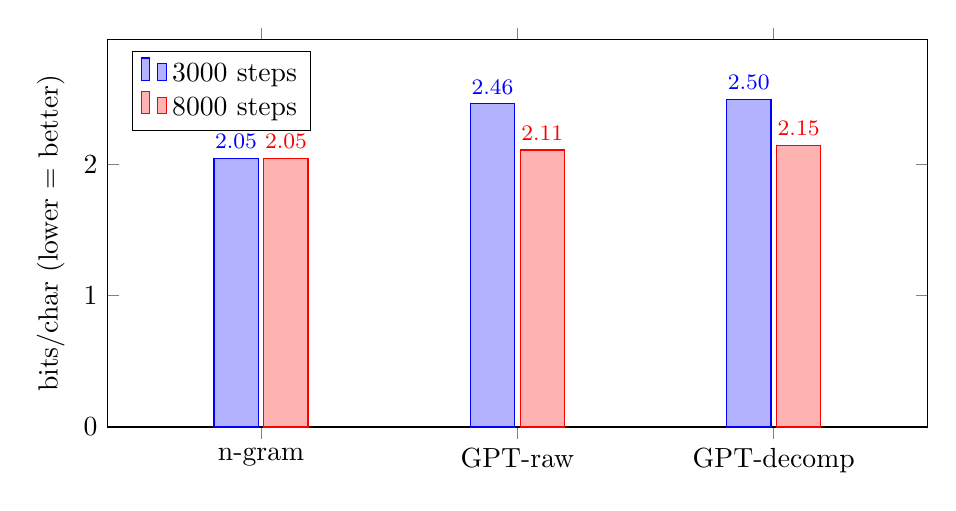
\begin{tikzpicture}
\begin{axis}[
  ybar, width=12cm, height=6.5cm,
  symbolic x coords={n-gram, GPT-raw, GPT-decomp},
  xtick=data, ylabel={bits/char (lower = better)},
  nodes near coords,
  every node near coord/.append style={font=\footnotesize,/pgf/number format/.cd,fixed,fixed zerofill,precision=2},
  ymin=0, ymax=2.95, bar width=16pt, enlarge x limits=0.3, legend pos=north west]
\addplot coordinates {(n-gram,2.0458) (GPT-raw,2.4613) (GPT-decomp,2.4961)};
\addplot coordinates {(n-gram,2.0458) (GPT-raw,2.1103) (GPT-decomp,2.1468)};
\legend{3000 steps, 8000 steps}
\end{axis}
\end{tikzpicture}
\caption{\textbf{Both gates negative, but robust.} The $n$-gram (memory) beats both transformers; decomposition
$\geq$ raw text. More training narrowed the GPT$\to$$n$-gram gap from $0.45$ to $0.10$ bits/char --- the transformer
\emph{almost} matches but does not cross the threshold.}
\end{figure}

\paragraph{Verdict.} \emph{Generalization:} $2.147 \geq 2.046$ --- \textbf{negative} (close). \emph{Ablation:}
$2.147 \geq 2.110$ --- \textbf{negative} (a stable $\sim$0.035 penalty at both 3000 and 8000). Generation samples:
the decomp model reproduces \emph{structure} (markers, section references, identifiers), the raw model reproduces
\emph{dialectical vocabulary}; both are locally plausible but globally incoherent --- they learned style and
skeleton, not meaning.

\section{Discussion --- why the mechanism works yet the result is negative}
\paragraph{This is not a failure of attention or gradient descent.} The model learned (loss decreased, learning
gate $55\times$). The bottleneck is \emph{information in the data}, not the mechanism.
\begin{enumerate}
  \item \textbf{Too little data.} $\sim$1M tokens for 2.64M parameters. The compute-optimal rule is $\sim$20
  tokens/parameter \cite{chinchilla} $\Rightarrow$ on the order of $50$M tokens needed; we are $\sim$20$\times$
  under-data'd.
  \item \textbf{Low entropy (repetition).} The vault shares a lot of boilerplate (section headers, domain
  vocabulary, identifiers). Effective information $\ll$ 3 MB; the $n$-gram simply \emph{memorizes} repeated strings,
  and the held-out (from the same projects) shares them.
  \item \textbf{Memory vs.\ generalization.} The $n$-gram is non-parametric memory (zero error on seen contexts);
  the transformer compresses lossily into fixed weights. On repetitive data exact memory beats lossy compression;
  the transformer's advantage (variable, long-range context) has nothing to reward it.
\end{enumerate}

\paragraph{Why decomposition does not help.} Markers add \emph{predictable} tokens (artificially lowering loss on
the decomp corpus) but no generalizable information about the language; evaluated on raw text they are
\emph{off-distribution} --- hence the stable penalty. Structure helps only as an \emph{inductive bias} aligned with
the task; for predicting the raw next character, dialectical markers are not such a bias.

\paragraph{Scope (honestly).} This result does \textbf{not} concern decomposition \emph{at inference time}
(breaking a task into trivial steps for a small model --- a distinct, separately validated mechanism). Nor is it a
general refutation of structure's value --- the test was conservative and micro-scale.

\paragraph{Redirection (data-driven).} Since the $n$-gram wins on memory and the transformer contributes
generalization, the principled move is to \emph{combine} them: \textbf{kNN-LM} \cite{knnlm} --- a transformer plus a
non-parametric nearest-neighbor datastore (like an $n$-gram, but in representation space; in the limit:
infini-gram \cite{infinigram}). Vault knowledge would then enter \emph{through the datastore, not the weights} ---
adding a note expands the model's memory with no retraining. The other route is adapting a \emph{pretrained} model
(which already knows the language), not training from scratch.

\section{Limitations (refutation conditions)}
\begin{itemize}
  \item \textbf{One base, one seed.} A result on one vault; replication on other corpora is open.
  \item \textbf{Conservative ablation.} The decomp model is evaluated on the raw held-out (off-distribution); the
  test favors raw. A decomp win would be all the stronger --- but there is none.
  \item \textbf{Micro scale.} The generalization gate is \emph{scale-dependent}: the narrowing gap
  $0.45\!\to\!0.10$ suggests a larger corpus/model/longer training could cross the threshold. To refute
  ``memory $\geq$ generalization'': exhibit a corpus/scale where GPT-decomp $<$ $n$-gram.
\end{itemize}

\section{Conclusions}
On a $\sim$3 MB structured knowledge base, a from-scratch micro-transformer \textbf{does not beat} a simple
$n$-gram (memory $\geq$ generalization), and dialectical decomposition does \textbf{not} build better
representations for modeling raw text --- and this is \emph{robust at convergence}, not an artifact of too-short
training (which we show by reporting both 3000 and 8000 steps). The mechanism (attention, gradient) is sound; we are
limited by information in the data (small + repetitive), consistent with scaling laws and the memory/generalization
trade-off. The most valuable negative is one that redirects effort: the data point to combining non-parametric
memory with generalization (kNN-LM) and adapting pretrained models --- rather than training micro knowledge-models
from scratch. Code, the corpus recipe, and the dialectical notes (thesis $\leftrightarrow$ antithesis $\to$
synthesis) are open in the repository.

\begin{thebibliography}{9}
\bibitem{vaswani} A.~Vaswani et al. \emph{Attention Is All You Need}. NeurIPS 2017.
\bibitem{nplm} Y.~Bengio et al. \emph{A Neural Probabilistic Language Model}. JMLR 2003.
\bibitem{knnlm} U.~Khandelwal et al. \emph{Generalization through Memorization: Nearest Neighbor Language Models}. ICLR 2020. arXiv:1911.00172.
\bibitem{infinigram} J.~Liu et al. \emph{Infini-gram: Scaling Unbounded $n$-gram Language Models to a Trillion Tokens}. COLM 2024. arXiv:2401.17377.
\bibitem{chinchilla} J.~Hoffmann et al. \emph{Training Compute-Optimal Large Language Models} (Chinchilla). NeurIPS 2022. arXiv:2203.15556.
\bibitem{graphrag} D.~Edge et al. \emph{From Local to Global: A Graph RAG Approach to Query-Focused Summarization}. arXiv:2404.16130, 2024.
\bibitem{argmining} J.~Lawrence, C.~Reed. \emph{Argument Mining: A Survey}. Computational Linguistics 45(4), 2019.
\bibitem{spektrum} A.~Słota. \emph{From $n$-gram to transformer: a spectrum of next-character prediction mechanisms}. Slayer collective, 2026.
\end{thebibliography}

\end{document}
